
\section*{Overview}

\RevBayes~has as a central idea that any statistical model, for example a phylogenetic model, is composed of smaller parts that can be decomposed and put back together in a modular fashion. This comes from considering (phylogenetic) models as \textit{probabilistic graphical models}, which lends flexibility and enhances the capabilities of the program. 
Users interact with \RevBayes~ via an interactive shell.
Users communicate commands using a language specifically designed for \RevBayes, called \Rev; an R-like language (complete with control statements, user-defined functions, and loops) that enables the user to build up (phylogenetic) models from simple parts (random variables, transformations, models, and constants of different sorts).
 

This tutorial demonstrates the basic syntactical features of \RevBayes~and \Rev~and shows to set up and perform an analysis on toy statistical models for linear regression. 
This tutorial focuses on explaining probabilistic graphical models and the language \Rev.
A good reference for probabilistic graphical models for Bayesian phylogenetic inference is given in \citep{hoehnaGM2014}.
The statistical examples are borrowed from a fourth year statistics course taught in the fall term 2011 at Stockholm University.


\bigskip
\subsection*{Probabilistic Graphical Models}

\RevBayes~uses \textit{probabilistic graphical models} for model specification, visualization, and implementation \citep{hoehnaGM2014}. 
Graphical models are frequently used in machine learning and statistics to visually represent the conditional dependence structure of complex statistical models with many parameters \citep{Gilks1994,lunn00,Jordan2004,Koller2009,Lunn2009}. 
The graphical model tool kit allows for flexible model specification and implementation and reduces redundant code. 
This framework provides a set of symbols for depicting a \href{http://en.wikipedia.org/wiki/Directed_acyclic_graph}{\textit{directed acyclic graph}} (DAG). 
\citet{hoehnaGM2014} described the use of probabilistic graphical models for phylogenetics. 
The different nodes and components of a phylogenetic graphical model are shown in Figure \ref{gmnotation} \citep[Fig. 1 from][]{hoehnaGM2014}. 
\begin{figure}[h!]
\centering
\fbox{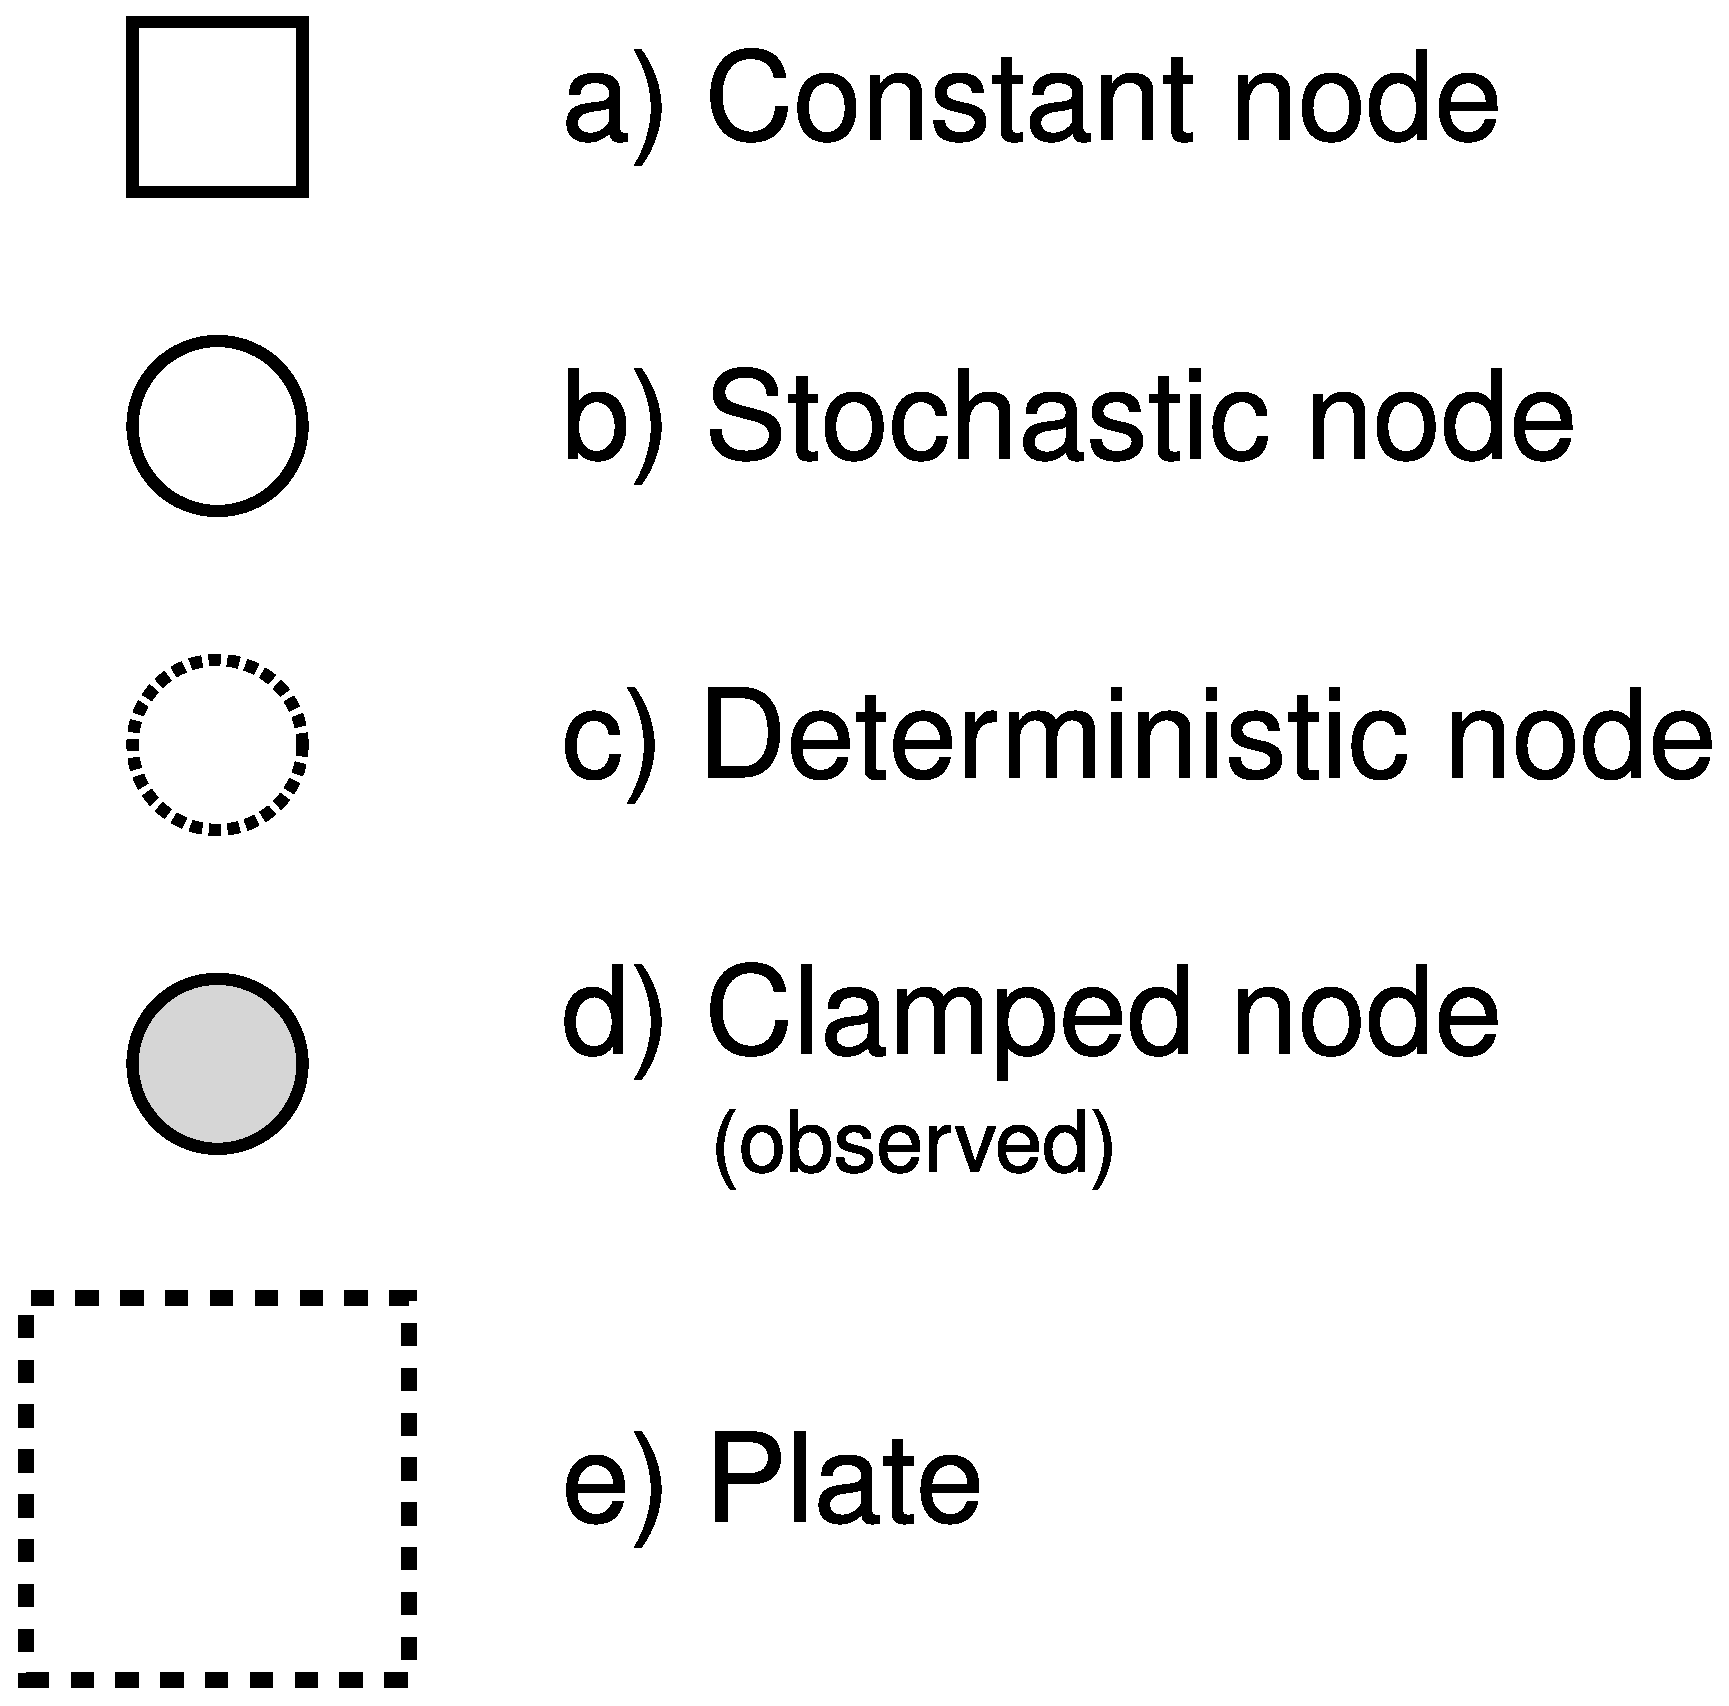
\includegraphics[width=1.8in,angle=0]{figures/GM_notation_figure.eps}}
\caption{\small The symbols for a visual representation of a graphical model. 
a) Solid squares represent constant nodes, which specify fixed-valued variables. 
b) Stochastic nodes are represented by solid circles. 
These variables correspond to random variables and may depend on other variables. 
c) Deterministic nodes (dotted circles) indicate variables that are determined by a specific function applied to another variable. 
They can be thought of as variable transformations. 
d) Observed states are placed in clamped stochastic nodes, represented by gray-shaded circles. e) Replication over a set of variables is indicated by enclosing the replicated nodes in a plate (dashed rectangle). 
[Partially reproduced from Fig.~1 in \citet{hoehnaGM2014}.]
}
\label{gmnotation}
\end{figure}

To represent the DAG, nodes are connected with arrows indicating dependency. 
A simple, albeit abstract, graphical model is shown in Figure \ref{simpleGM}. 
In this model, we observe a set of states for parameter $x$. 
We assume that the values of $x$ are samples from a lognormal distribution with a location parameter (log mean) $\mu$ and a standard deviation $\sigma$. 
It is more straightforward to model our uncertainty in the expectation of a lognormal distribution, rather than $\mu$, thus we place a gamma distribution on the mean $M$. 
This gamma hyperprior has two parameters that we specify with fixed values (constant nodes): the shape $\alpha$ and rate $\beta$. 
With this prior density, the variable $M$ is a stochastic node.
The standard deviation, $\sigma$, is also a stochastic node with an exponential prior density with rate parameter $\lambda$.
For any value of $M$ and any value of $\sigma$ we can compute the deterministic variable $\mu$ using the formula $\mu = \ln(M) - \frac{\sigma^2}{2}$. 
This formula is known from using simple algebra on the equation for the mean of any \href{http://en.wikipedia.org/wiki/Log-normal_distribution}{lognormal distribution}.
With this model structure, we can then calculate the probability of the data conditional on the model (the likelihood): 
$\mathbb{P}(\boldsymbol{x} \mid \mu, \sigma)$. With this, we can get the posterior probability using Bayes' theorem:
$$\mathbb{P}(M,\sigma \mid \boldsymbol{x}, \alpha, \beta, \lambda) = \frac{\mathbb{P}(\boldsymbol{x} \mid \mu, \sigma) \mathbb{P}(M \mid \alpha,\beta) \mathbb{P}(\sigma \mid \lambda)}{\mathbb{P}(\boldsymbol{x})}.$$
\begin{figure}[h!]
\centering
\fbox{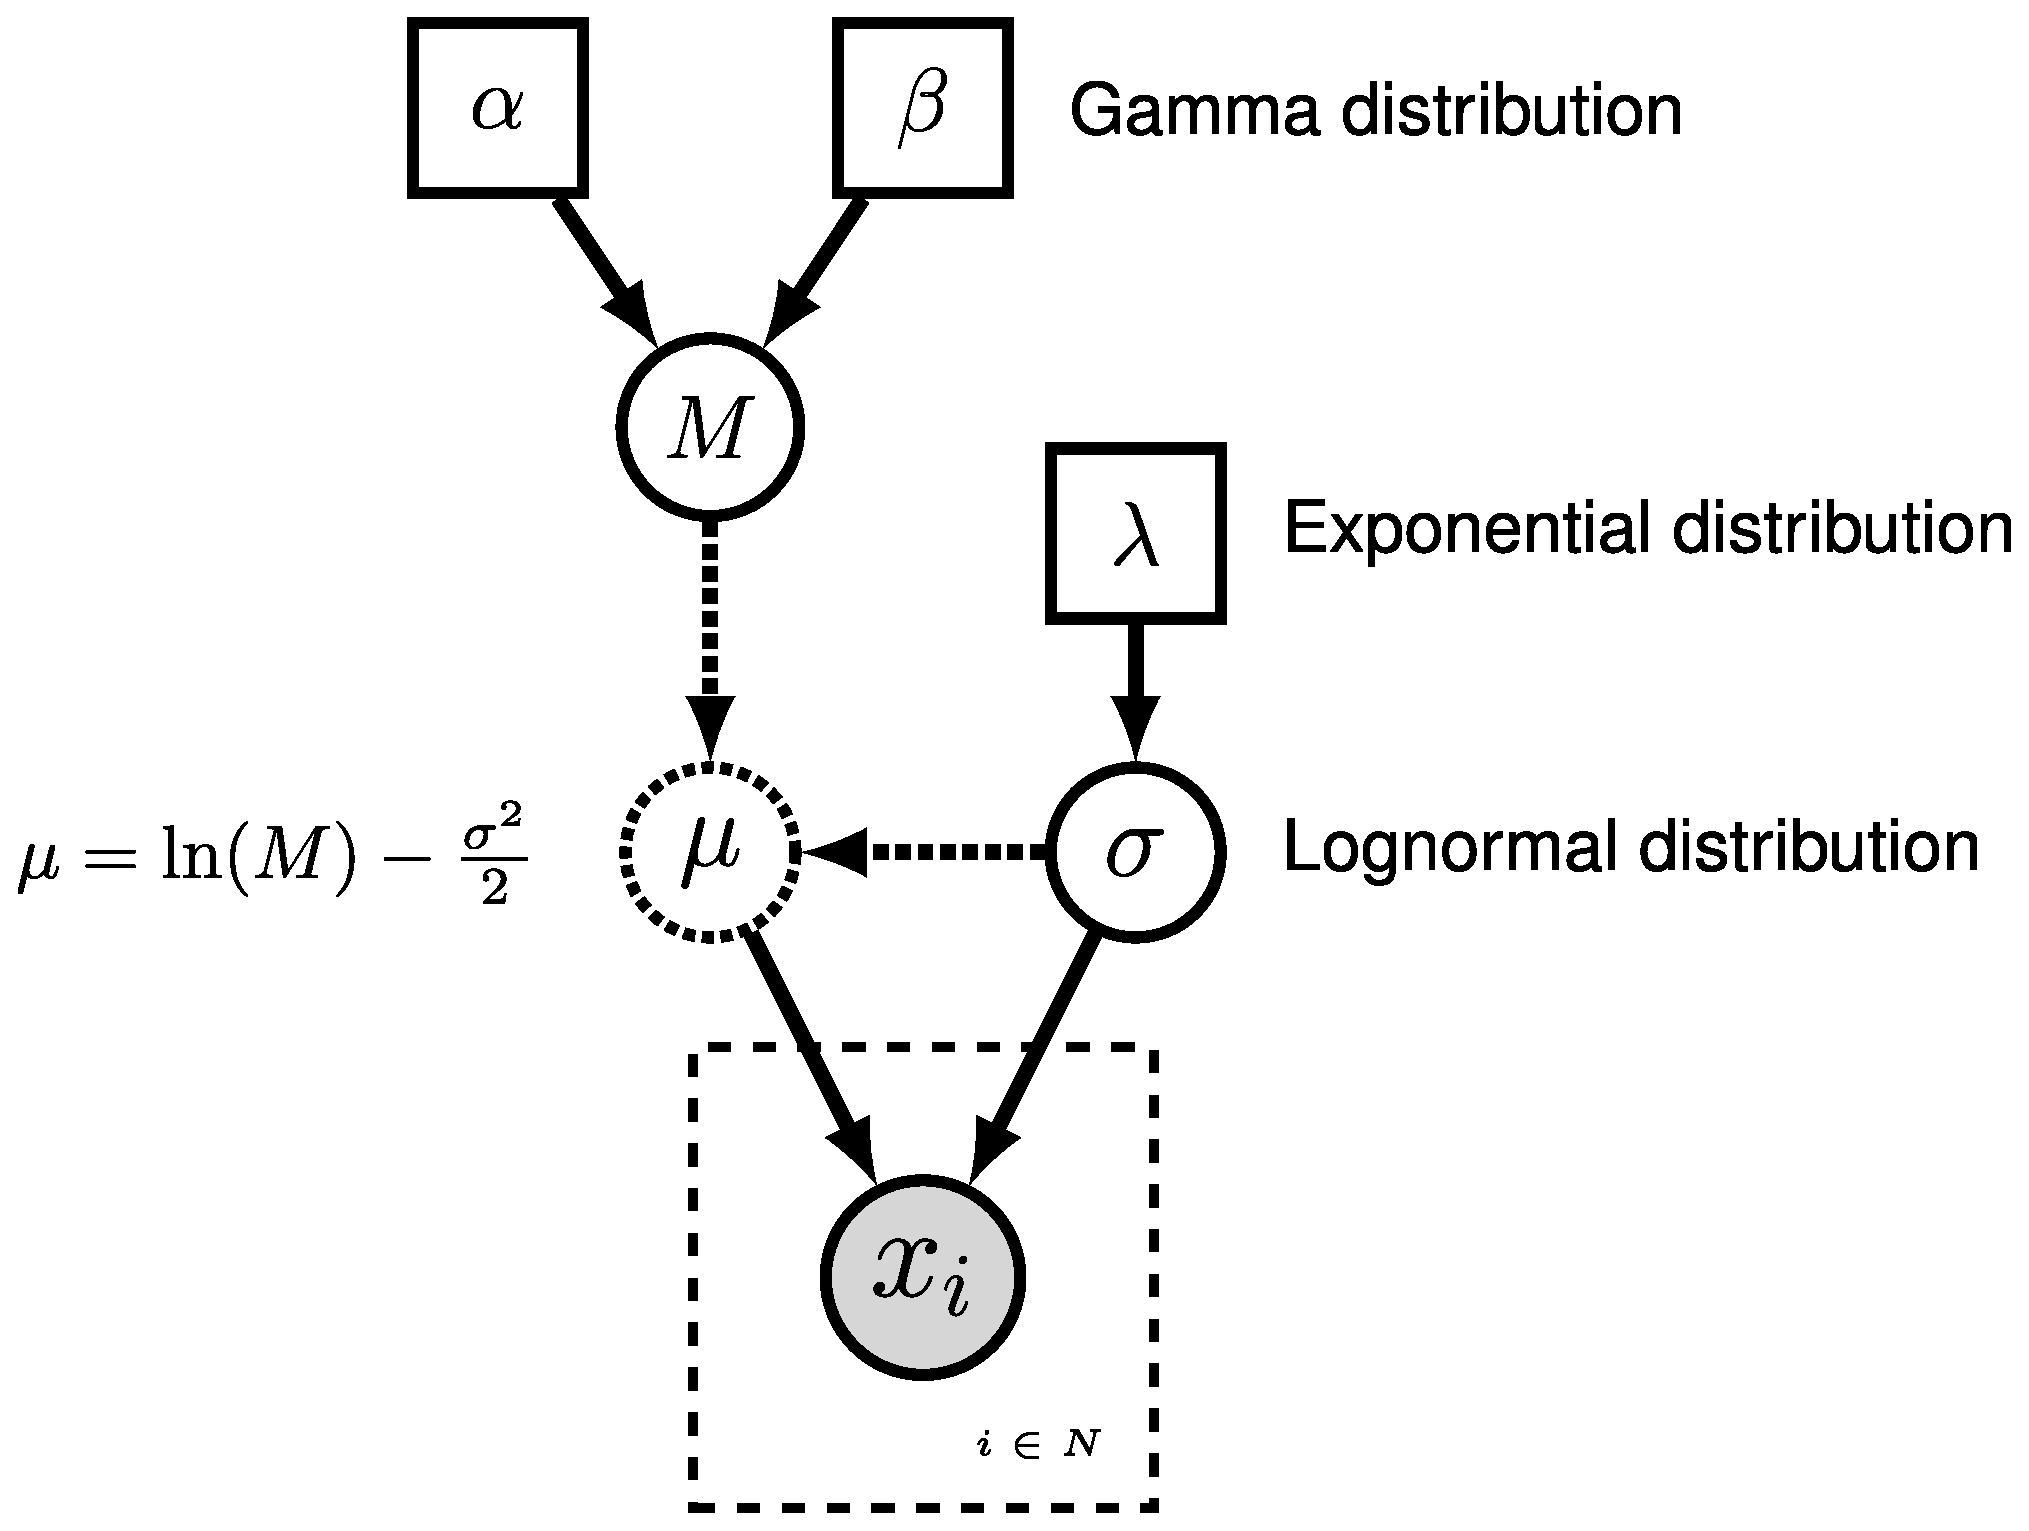
\includegraphics[width=2.5in,angle=0]{figures/simple_GM.eps}}
\caption{\small Graphical model representation of a simple lognormal model. A total of $N$ states of parameter $x$ are observed and occupy a clamped node. 
This parameter is log-normally distributed with parameters $\mu$ and $\sigma$ (log mean and standard deviation, respectively). 
The parameter $\mu$ is a deterministic node that is calculated from the stochastic nodes $M$ (the mean of the distribution) and $\sigma$. 
Dotted arrows indicate deterministic functions and are used to connect deterministic nodes to their parent variables. 
A gamma distribution is applied as a hyper prior on $M$ with constant nodes for the shape $\alpha$ and rate $\beta$. 
The stochastic variable $\sigma$ is exponentially distributed with fixed value for the rate $\lambda$.
}
\label{simpleGM}
\end{figure}



\bigskip
\subsection*{The \Rev~Language}

In \RevBayes~models and analyses are specified using an interpreted language called \Rev. 
\Rev~bears similarities to the compiled language in WinBUGS and the interpreted \R~language. 
Setting up and executing a statistical analysis in \RevBayes~requires the user to specify all of the parameters of their model and the type of analysis (e.g., an MCMC run). 
By using an interpreted language, \RevBayes~enables the practitioner to build complex, hierarchical models and to check the current states of variables while building the model. 

Differently to \R~and BUGS, \Rev~is a strongly but implicitly typed language.
It is implicitly typed, and thus similar to Python, because you do not need to provide the type of a variable (which you need to in language such as C++ and Java).
We do implicit typing to help users who do not know about the actual types of the variables.
However, strongly typed means that every variable has a type and arguments of functions need to match the required types.
The strong type requirements ensures that you build meaningful model graphs. 
For example, the variance parameter of a normal distribution needs to be a positive number, and thus you can only use variables that are positive real numbers.
We do automatic type conversion, although some parts of it are still under construction.

\bigskip
\subsubsection*{Specifying Models}

\begin{table}[h!]
\centering
\caption{Rev language node assignment operators, clamp function, and plate/loop syntax.}\label{operatorTable}
\begin{tabular}{@{\extracolsep{\fill}}l  c r }
\hline
\multicolumn{1}{l}{\textbf{Operator}} & \multicolumn{1}{c}{ } & \multicolumn{1}{r}{\textbf{Node}}  \\ 
\hline
\cl{<-} & \hspace{10mm} &  constant node\\
\cl{\rbdn} & \hspace{10mm} &  stochastic node\\
\cl{:=} & \hspace{10mm} &  deterministic node\\
\cl{node.clamp(data)} & \hspace{10mm} &  clamped node\\
\cl{for(i in 1:N)\{...\}} & \hspace{10mm} &  plate\\
\hline
\end{tabular}
\end{table}

The nodes representing parameters of a statistical model are created using different operators in \Rev~(Table \ref{operatorTable}). 
In Figure \ref{revgmexample}, the \Rev~syntax for creating the model in Figure \ref{simpleGM} is provided.
Because \Rev~is an interpreted language, it is important to consider the order in which you specify your model (cf. BUGS where the order is not important). 
Thus, typically the first nodes that are instantiated are \emph{constant nodes}. 
Constant nodes require you to assign a fixed value to the parameter using the \cl{<-} operator. 
Stochastic nodes are initialized using the \cl{\rbdn} operator followed by the constructor function for a distribution. 
In \Rev, the naming convention for distributions is \cl{dn*}, where \cl{*} is a wildcard representing the name of the distribution. 
Each distribution function requires hyperparameters passed in as arguments. 
This is effectively linking nodes using arrows in the graphical model.
The following code snippet creates a stochastic node called \cl{M} which is assigned a gamma-distributed hyperprior, with shape \cl{alpha} and rate \cl{beta}:
{\tt \begin{snugshade*}
\begin{lstlisting}
alpha <- 2.0
beta <- 4.0
M ~ dnGamma(alpha, beta)
\end{lstlisting}
\end{snugshade*}}

The flexibility gained from the graphical model framework and the interpreted language allows you to easily change a model by swapping components. 
For example, if you decide that a bimodal lognormal distribution is a better representation of your uncertainty in \cl{M}, then you can simply change the distribution associated with \cl{M} (after initializing the bimodal lognormal hyperparameters):
{\tt \begin{snugshade*}
\begin{lstlisting}
mean_1 <- 0.5
mean_2 <- 2.0
sd_1 <- 1.0
sd_2 <- 1.0
weight <- 0.5
M ~ dnBimodalLdnNorm(mean_1, mean_2, sd_1, sd_2, weight)
\end{lstlisting}
\end{snugshade*}}

\Rev~does allows you to specify constant-node values in the distribution constructor function, therefore this also works:
{\tt \begin{snugshade*}
\begin{lstlisting}
M ~ dnBimodalLdnNorm(0.5, 2.0, 1.0, 1.0, 0.5)
\end{lstlisting}
\end{snugshade*}}



\begin{figure}[h!]
\centering
\fbox{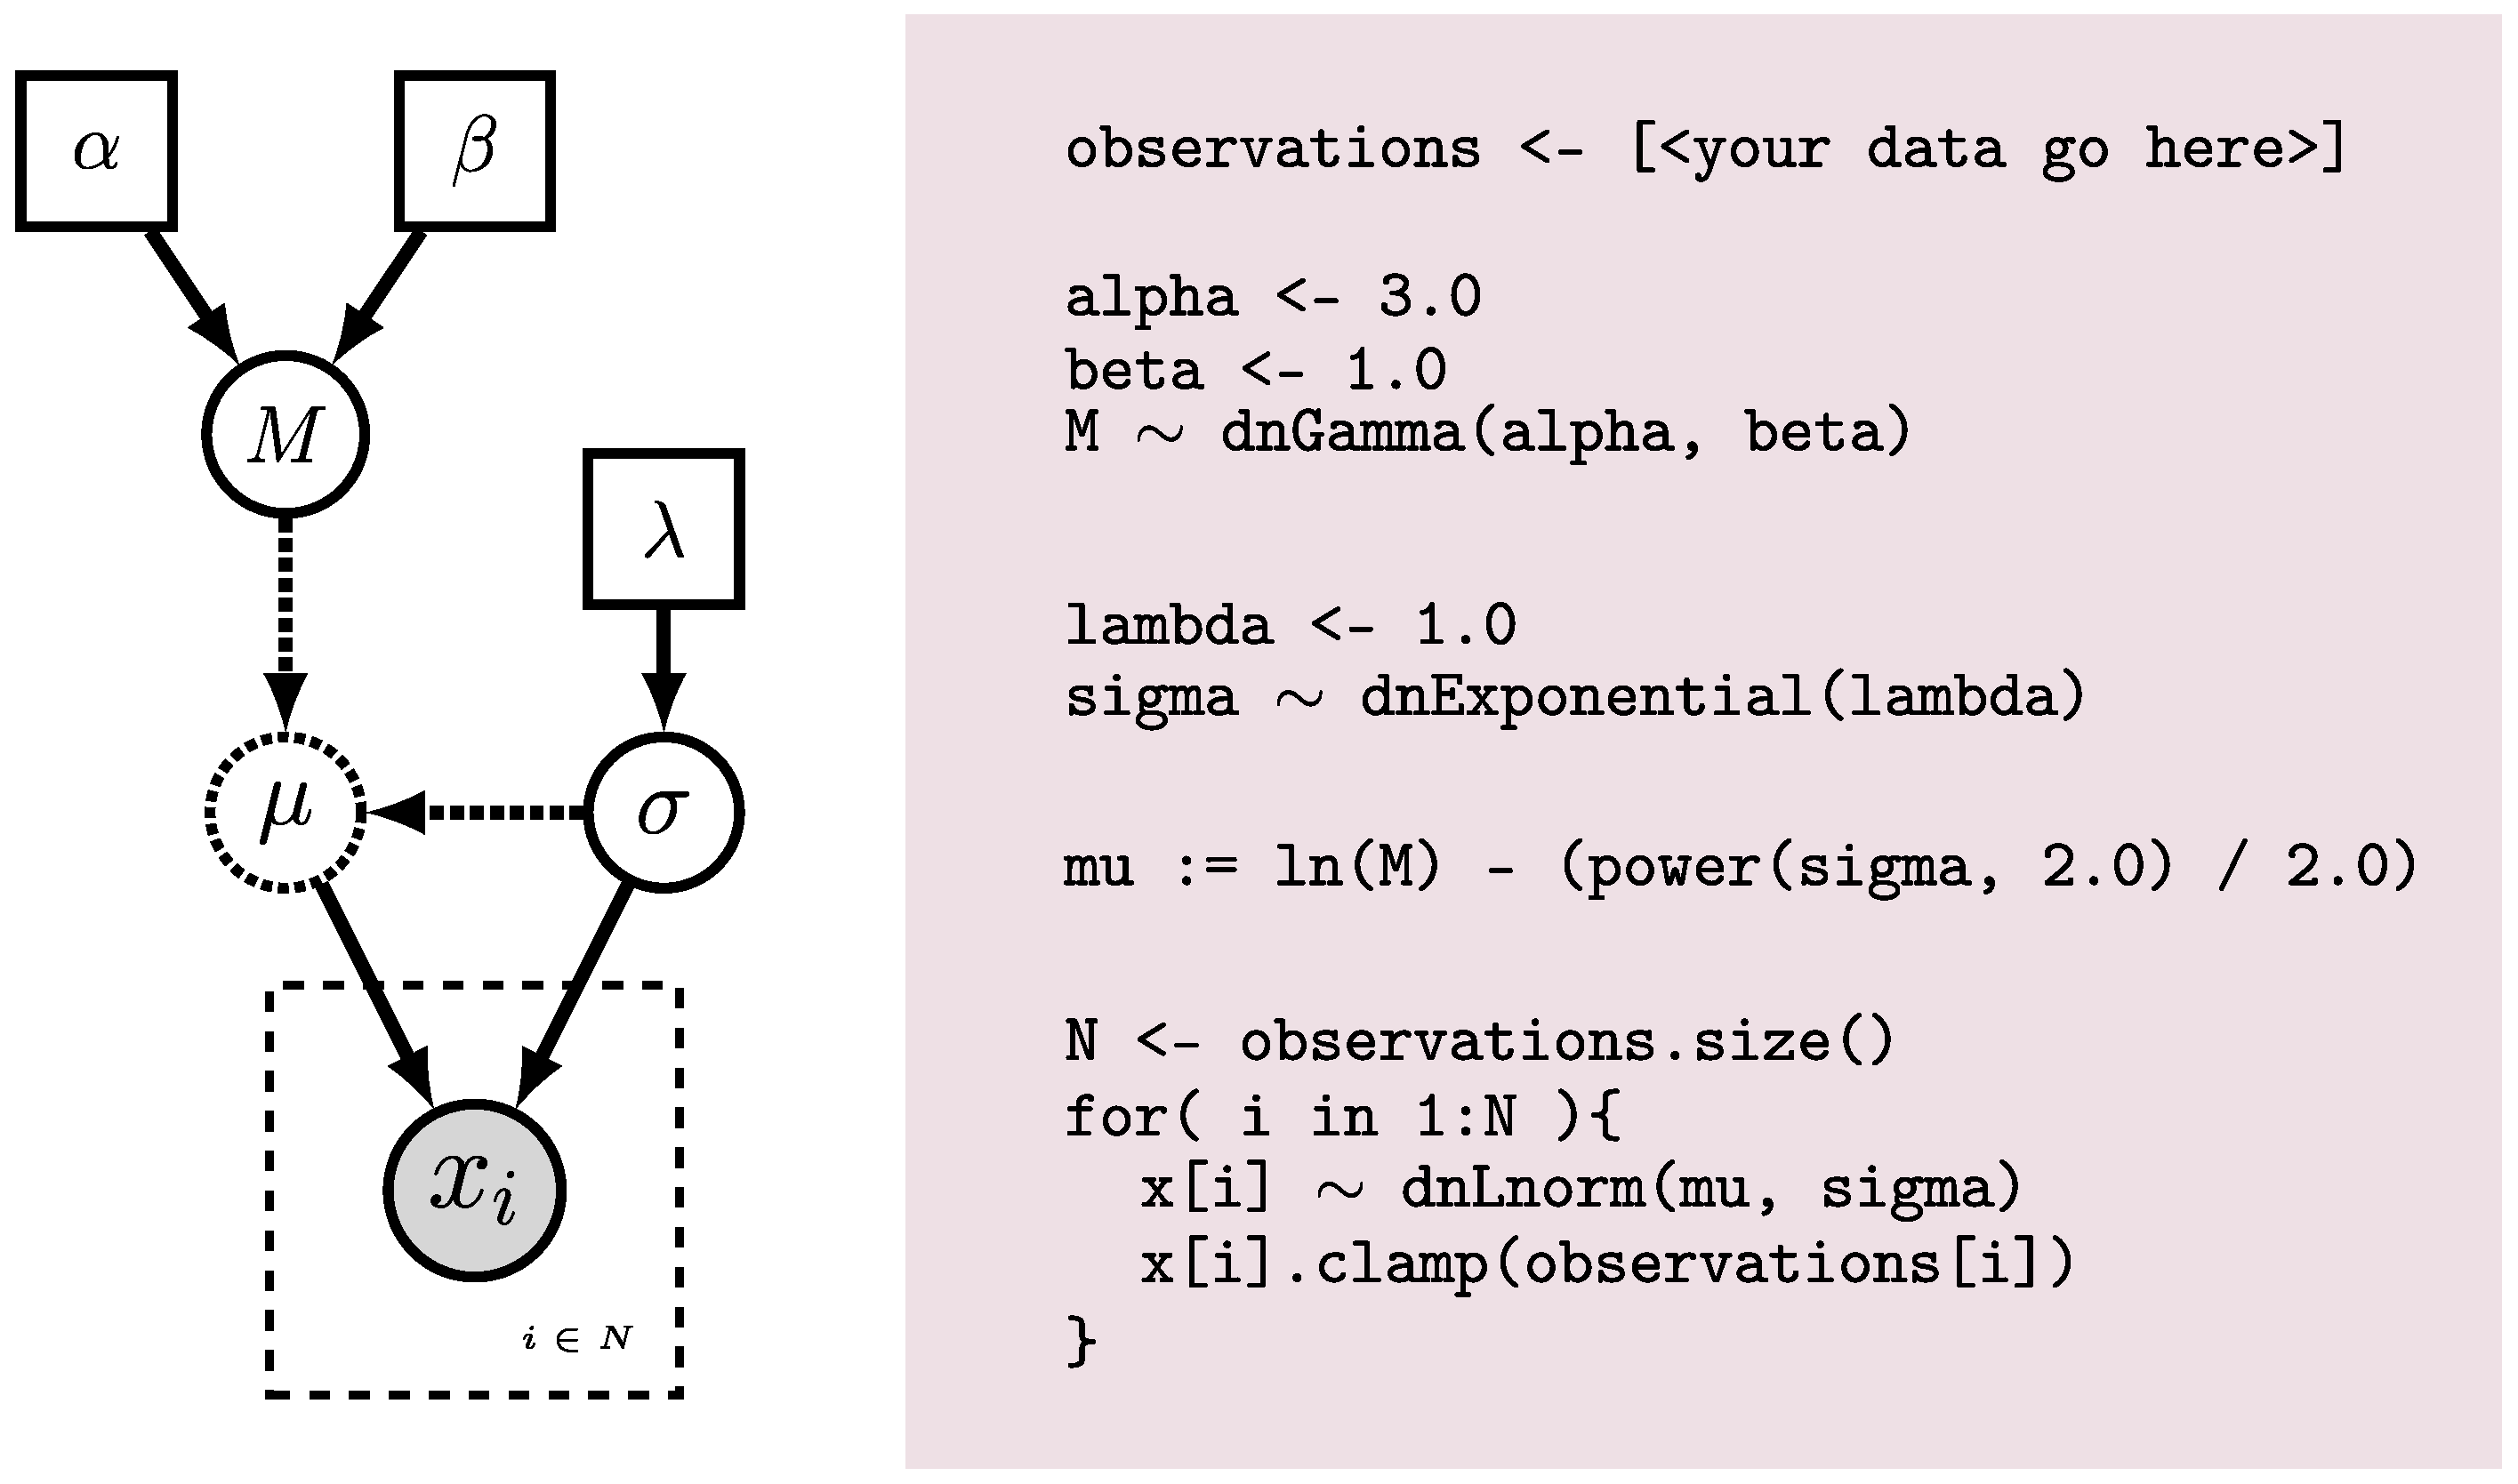
\includegraphics[width=5in,angle=0]{figures/simple_GM_rev.eps}}
\caption{\small Specifying a model with \Rev. 
The graphical model of the observed parameter $x$ is shown on the left. 
In this example, $x$ is log-normally distributed with a location parameter of $\mu$ and a standard deviation of $\sigma$, thus $x \sim \mbox{Lognormal}(\mu, \sigma)$. 
The expected value of $x$ (or mean) is equal to $M$: $\mathbb{E}(x) = M$. 
In this model, $M$ and $\sigma$ are random variables and each are assigned hyperpriors. 
We assume that the mean is drawn from a gamma distribution with shape parameter $\alpha$ and rate parameter $\beta$: $M \sim \mbox{Gamma}(\alpha, \beta)$. 
The standard deviation of the lognormal distribution is assigned an exponential hyperprior with rate $\lambda$: $\sigma \sim \mbox{Exponential}(\lambda)$. 
Since we are conditioning our model on the \emph{expectation}, we must compute the location parameter ($\mu$) to 
calculate the probability of our model. 
Thus, $\mu$ is a deterministic node that is the result of the function$^*$ executed on $M$ and $\sigma$: $\mu = \ln(M) - \frac{\sigma^2}{2}$. 
Since we observe values of $x$, we \emph{clamp} this node.
}
\label{revgmexample}
\end{figure}

Deterministic nodes are variable transformations and initialized using the \cl{:=} operator followed by the function or formula for calculating the value. 
Thus, if you had an exponentially distributed stochastic node and you also wanted to monitor the square root of that variable, you can create a deterministic node:
{\tt \begin{snugshade*}
\begin{lstlisting}
p ~ dnExponential(1.0)
sq_p := sqrt(p)
\end{lstlisting}
\end{snugshade*}}

Replication over lists of variables as a plate object is specified using \cl{for} loops. 
A for-loop is an iterator statement that performs a function a given number of times. 
In \Rev~you can use this syntax to create a vector of 12 stochastic nodes, each drawn from a Poisson distribution:
{\tt \begin{snugshade*}
\begin{lstlisting}
rate <- 2.5
for( i in 1:12 ){
  p[i] ~ dnPoisson(rate)
}
\end{lstlisting}
\end{snugshade*}}

A clamped node is attached to observed data. 
Thus, you must first read in or input the data as a constant node, then clamp it to a stochastic node. 
In Figure \ref{revgmexample} the observations are assigned and clamped to the stochastic nodes.
If we observed 7 values for \cl{x} we would create 7 clamped nodes:
{\tt \begin{snugshade*}
\begin{lstlisting}
observations <- [0.20, 0.21, 0.03, 0.40, 0.65, 0.87, 0.22]
N <- observations.size()
for( i in 1:N ){
  x[i] ~ dnLognormal(mu, sigma)
  x[i].clamp(observations.clamp)
}
\end{lstlisting}
\end{snugshade*}}



\subsection*{Getting help in \RevBayes}
%\taha{will there be help information by this time?}
%
%This displays a list of the different elements and commands available in RevBayes. The \cl{help} command also provides more detailed information about each of these items.
%
%For example, we can view the \cl{help()} information about the \cl{log()} function:
%


Currently, the help-system of \RevBayes~is virtually nonexistent. 
This will not always be the case, but is par for the course when using new/experimental software. 
The most complete help file available is for the \cl{mcmc()} function. Display the help for this function using the \cl{?} symbol:
{\tt \begin{snugshade*}
\begin{lstlisting}
RevBayes > ?mcmc
\end{lstlisting}
\end{snugshade*}}

Additionally, \RevBayes~will print the correct usage of a function if it is executed without any arguments:
{\tt \small \begin{snugshade*}
\begin{lstlisting}
RevBayes > mcmc()
   Error:   Argument mismatch for call to function 'mcmc'( ). Correct usage is:
   MCMC function (Model model, VectorRbPointer<Monitor> monitors,
   VectorRbPointer<Move> moves, String moveschedule = sequential|random|single)
\end{lstlisting}
\end{snugshade*}}

%allows you to save all of the screen output from your analysis to a log file. 
%The \cl{help} information for this command displays all of the available options for specifying screen logging.
%We are going to log our screen output to a file called \cl{conifer-partn-log.txt}.
%\mbcl{log start filename=conifer-partn-log.txt}
%
%Next, load the sequences into the program using the \cl{execute} command.
%\mbcl{execute conifer\_dna.nex}



\vspace{5mm}

{\begin{framed}
\begin{center}
Continue on to the next page to start the exercise...
\end{center}
\end{framed}}






%
%\subsection*{Analysis Functions}
%
\newpage
\FloatBarrier
\section{Exercise: Basic Rev Commands}

\subsection{Introduction}

The first section of this exercise involves 
\begin{enumerate}
\item Creating different types of variables.
\item Learning about functions. 
\end{enumerate}

All of the files for this analysis are provided for you and you can run these without significant effort using the \cl{source()} function in the \RevBayes~console:
{\tt \begin{snugshade*}
\begin{lstlisting}
RevBayes > source("RevBayes_scripts/basics.Rev")
\end{lstlisting}
\end{snugshade*}}


Let's start with the basic concepts for the interactive use of \RevBayes~with \Rev~(the language of \RevBayes). 
You should try to execute the statements step by step, look at the output and try to understand what and why things are happening. 
We start with some simple concepts to get familiar and used to \RevBayes. 
By now you should have executed \RevBayes~and you should see the command prompt waiting for input. 
The best exercise is to write these statements exactly in \RevBayes. 

\Rev~is an interpreted language for statistical computing and analyses in evolutionary biology. Therefore, the basics are simple mathematical operations, such as 
{\tt \begin{snugshade*}
\begin{lstlisting}    
> # Simple mathematical operators:
> 1 + 1                            # Addition
> 10 - 5                           # Subtraction
> 5 * 5                            # Multiplication
> 10 / 2                           # Division
> 2^3                              # Exponentiation
> 5%2                              # Modulo
\end{lstlisting}
\end{snugshade*}}
Just as a side note, you can also write multiple statements in the same line if you separate these by \cl{;}.
The statements will be executed as if you wrote each on a single line.
{\tt \begin{snugshade*}
\begin{lstlisting}    
> 1 + 1; 2 + 2                    # Multiple statements in one line
\end{lstlisting}
\end{snugshade*}}
    
Here you can see that comments always start with the symbol `\cl{\#}'. 
Everything after the `\cl{\#}'-symbol will be ignored.
In addition to these simple mathematical operations, we provide some standard math functions which can be called by:
    
{\tt \begin{snugshade*}
\begin{lstlisting}    
> # Math-Functions
> exp(1)                           # exponential function
> ln(1)                            # logarithmic function with natural base
> sqrt(16)                         # square root function 
> power(2,2)                       # power function: power(a,b) = a^b
\end{lstlisting}
\end{snugshade*}}
Notice that \Rev~is case-sensitive. That means \Rev~distinguishes upper and lower case letterd for both variable names and function names. For example, only the first of these two calls will work
{\tt \begin{snugshade*}
\begin{lstlisting}    
> exp(1)                           # correct lower case name
> Exp(1)                           # wrong upper case name
\end{lstlisting}
\end{snugshade*}}
Moreover, we provide functions for the common statistical distributions.
{\tt \begin{snugshade*}
\begin{lstlisting}    
> # distribution functions
> dexp(x=1,rate=1)         # exponential distribution density function
> qexp(0.5,1)              # exponential distribution quantile function
> rexp(n=10,1)             # random draws from an exponential distribution
> ddnNorm(-2.0,0.0,1.0)              # normal distribution density function
> rdnNorm(n=10,0,1)                  # random draws from a normal distribution
\end{lstlisting}
\end{snugshade*}}
If you do not remember what the parameter or parameter names of a function are, then you can simply type in the function name and \RevBayes~will tell you the possible parameters with their names.
{\tt \begin{snugshade*}
\begin{lstlisting}    
> rexponential
\end{lstlisting}
\end{snugshade*}}

The next, and very important feature of \RevBayes~is variable declaration. 
We have three types of variables, namely constant, deterministic and stochastic variables, which represent the same three types of DAG nodes. 
Here we show how to construct the different variables and how they behave differently. 
First, we focus on the difference between constant and deterministic variables: 

First, we create a constant variable with name \cl{a} and assigned the value 1 to it. 
The left arrow assignment (\cl{<-}) will always create a constant variable.
{\tt \begin{snugshade*}
\begin{lstlisting}    
> # Variable assignment: constant and deterministic
> a <- 1                           # assignment of constant node 'a'
\end{lstlisting}
\end{snugshade*}}
You see the value of 'a' by just typing in the variable name and pressing enter.
{\tt \begin{snugshade*}
\begin{lstlisting}    
> a                                # printing the value of 'a'
\end{lstlisting}
\end{snugshade*}}
If you want to see which type of variable (constant, deterministic or stochastic) 'a' has, then call the structure function for it.
{\tt \begin{snugshade*}
\begin{lstlisting}    
> str(a)                           # printing the structure information of 'a'
\end{lstlisting}
\end{snugshade*}}
An additional quite useful built-in function in \RevBayes~ is the \cl{type} function which gives you only the type information of the variable and thus is a subset of the \cl{str} function.
{\tt \begin{snugshade*}
\begin{lstlisting}    
> type(a)                          # printing the type information of 'a'
\end{lstlisting}
\end{snugshade*}}

Next, we created a deterministic variable computed by \cl{:=} and another deterministic variable \cl{c} computed by \cl{ln(b)}. 
Deterministic variables are always created using the colon-equal assignment (\cl{:=}). 

{\tt \begin{snugshade*}
\begin{lstlisting}    
> b := exp(a)                      # assignment of deterministic node 'b' with the exponential function with parameter 'a'
> b                                # printing the value of 'b'
> c := ln(b)                       # assignment of deterministic node 'c' with logarithmic function with parameter 'b'
> c                                # printing the value of 'c'
\end{lstlisting}
\end{snugshade*}}
Again, you see the type of the variable and additional information such as which the parents and children are by calling the structure function on it.
{\tt \begin{snugshade*}
\begin{lstlisting}    
> str(b)                           # printing the structure information of 'b'
\end{lstlisting}
\end{snugshade*}}
For example, see the difference to the creation of variable 'd', which is a constant variable.
{\tt \begin{snugshade*}
\begin{lstlisting}    
> d <- ln(b)                       # assignment of constant node 'd' with the value if the logarithmic function with parameter 'b'
> d                                # printing the value of 'd'
> str(d)                           # printing the structure information of 'd'
\end{lstlisting}
\end{snugshade*}}
Currently, the variables \cl{c} and \cl{d} have the same value. 
We can check this using the equal comparison (\cl{==}).
{\tt \begin{snugshade*}
\begin{lstlisting}    
> e := (c == d)			
> e
\end{lstlisting}
\end{snugshade*}}
Now, if we assign a new value to variable \cl{a}, then naturally the value of \cl{a} changes. 
This has the consequence that all deterministic variables that use 'a' as a parameter, i.e., the variable \cl{b}, change their value automatically too.
{\tt \begin{snugshade*}
\begin{lstlisting}    
> a <- 2                           # reassignment of variable a; every deterministic node which has 'a' as a parameter changes its value
> a                                # printing the value of 'a'
> b                                # printing the value of 'b'
> c                                # printing the value of 'c'
> d                                # printing the value of 'd'
> e
\end{lstlisting}
\end{snugshade*}}
Since variable \cl{d} was a constant variable it did not change its value. 

Finally, we show you how to create the third type of variables in \Rev: the stochastic variables. 
We will create a random variable \cl{x} from an exponential distribution with parameter \cl{lambda}.  
Stochastic assignments use the \cl{\rbdn} operation.
{\tt \begin{snugshade*}
\begin{lstlisting}    
> # Variable assignment: stochastic
> lambda <- 1                      # assign constant node 'lambda' with value '1'
> x ~ dnExponential(lambda)        # create stochastic node with exponential distribution and parameter 'lambda'
\end{lstlisting}
\end{snugshade*}}
The value of \cl{x} is a random draw from the distribution. 
You can see the value and the probability (or log-probability) of the current value under the current parameter values by
{\tt \begin{snugshade*}
\begin{lstlisting}    
> x                                # print value of stochastic node 'x'
> x.probability                    # print the probability if 'x'
> x.lnProbability                  # print the log-probability if 'x'
> str(x)                           # printing all the information of 'x'
\end{lstlisting}
\end{snugshade*}}
Similarly, we create a random variable \cl{y} from a normal distribution by
{\tt \begin{snugshade*}
\begin{lstlisting}    
> mu <- 0
> sigma <- 1
> y ~ dnNorm(mu,sigma)	
> y.probability                    # print the probability of 'y'
> y.lnProbability                  # print the log-probability if 'y'
> str(y)                           # printing all the information of 'y'
\end{lstlisting}
\end{snugshade*}}
Now you know everything there is about creating the different types of variables and the different ways in which these variables behave.



\subsubsection*{Simple variable manipulation and other types of assignments}
\Rev~provides some convenience variable manipulation operations that are equivalent to variable manipulations in other programming languages such as C/C++, Java and Python.
You can increment (\cl{++}) and decrement (\cl{--}) a variable.
The increment operation increases the current value of a variable by 1 and the decrement operation decreases the value by 1.
A post increment (\cl{a++}) increases the value after returning the value, that is, the old value is returned.
A pre increment (\cl{++a}) increases the value before returning the value, that is, the new value is returned.
Note that currently both the post- and pre-increment operations use a pre-increment functionality.
{\tt \begin{snugshade*}
\begin{lstlisting}    
> index <- 1
> index++                          # post increment
> ++index                          # pre increment
> index--                          # post decrement
> --index                          # pre decrement
\end{lstlisting}
\end{snugshade*}}
Additionally, you can use addition (\cl{a += b}), subtraction (\cl{a -= b}), multiplication (\cl{a *= b}) and division (\cl{a /= b}) to an existing variable.
{\tt \begin{snugshade*}
\begin{lstlisting}    
> index += 10                      # add 10 to the current value
> index *= 2                       # double the current value
\end{lstlisting}
\end{snugshade*}}
These variable manipulations will come in very handy for indices of vectors/arrays.

\subsubsection*{Vectors}
Common values in \RevBayes~are of scalar types.
That means, that not everything is a vector by default.
Instead, you can create a vector using three different ways.
First, you can call the vector function.
{\tt \begin{snugshade*}
\begin{lstlisting}    
> v <- v(1,2,3)                    # create a vector
\end{lstlisting}
\end{snugshade*}}
Interestingly, we can use the same name for a variable as for a function: the variable \cl{v} and the function \cl{v(\ldots)}.
Both will still be fully functional and our interpreter checks if you asked for a function or a variable.

Second, you can use the square bracket notation.
{\tt \begin{snugshade*}
\begin{lstlisting}    
> w <- [1,2,3]                     # create a vector
\end{lstlisting}
\end{snugshade*}}
And third, you can implicitly create the vector by assigning elements.
{\tt \begin{snugshade*}
\begin{lstlisting}    
> z[1] <-1                         # implicit creation of a vector
> z[2] <-2                   
> z[3] <-3                  
\end{lstlisting}
\end{snugshade*}} 
The implicit creation does not need to instantiate the variable beforehand.
There are other useful built-in functions that produce vectors.
{\tt \begin{snugshade*}
\begin{lstlisting}    
> 1:10                             # range function
> rep(10,1)                        # replicate an element n times
> seq(1,20,2)                      # built a sequence from a to b by c
\end{lstlisting}
\end{snugshade*}} 

Vectors in \Rev~belong to the class of objects that have members and/or methods.
You can get the member of such a member-object by calling
{\tt \begin{snugshade*}
\begin{lstlisting}    
> x.<member name>
\end{lstlisting}
\end{snugshade*}} 
Similarly, you can call a member method by
{\tt \begin{snugshade*}
\begin{lstlisting}    
> x.<member name>(<arguments>)                 
\end{lstlisting}
\end{snugshade*}} 
If you don't remember what the methods were called, or if this object has any member methods, then you can get these by
{\tt \begin{snugshade*}
\begin{lstlisting}    
> v.methods()                 
\end{lstlisting}
\end{snugshade*}} 
In general, this is very, very useful.
So for a vector we can get the size --- the number of elements --- by calling its member function:
{\tt \begin{snugshade*}
\begin{lstlisting}    
> v.size()                 
\end{lstlisting}
\end{snugshade*}} 


\subsubsection*{Control Structures}
In this next part we will learn about control structures in \Rev. 
The first control structure that we will look at is the \cl{for} loop.
\cl{for} loop execute a single statement or a block of 
{\tt \begin{snugshade*}
\begin{lstlisting}    
> # loops
> for (<variable> in <set of value>) <single statement>
> 
> for (<variable> in <set of value>) 
> <single statement>
>
> for (<variable> in <set of value>) {
> <multiple statements>
> <multiple statements>
> <multiple statements>
> }
\end{lstlisting}
\end{snugshade*}}
The statement(s) will be execute for each value of variable of the \cl{for} loop.
A simple example is a \cl{for} loop that computes the sum of 
{\tt \begin{snugshade*}
\begin{lstlisting}    
> sum <- 0
> for (i in 1:100) {
> sum <- sum + i
> }
> sum
\end{lstlisting}
\end{snugshade*}}
Another example using a \cl{for} loop is the computation of the \href{http://en.wikipedia.org/wiki/Fibonacci_number}{Fibonacci number} for a given integer. 
{\tt \begin{snugshade*}
\begin{lstlisting}    
> # Fibonacci series using a for loop
> fib[1] <- 1
> fib[2] <- 1
> for (j in 3:10) {
> fib[j] <- fib[j - 1] + fib[j - 2]
> }
> fib
\end{lstlisting}
\end{snugshade*}}
We could also compute the Fibonacci numbers using a \cl{while} loop.
The \cl{while} loop continues to execute the statement(s) until the condition is wrong.
{\tt \begin{snugshade*}
\begin{lstlisting}    
> # Fibonacci series using a while loop
> fib[1] <- 1
> fib[2] <- 1
> j <- 3
> while (j <= 10) {
> fib[j] <- fib[j - 1] + fib[j - 2]
> j++
> }
> fib
\end{lstlisting}
\end{snugshade*}}

\subsubsection*{User Defined Functions}
In \Rev~you can write your own functions as well.
The syntax for writing function is:
{\tt \begin{snugshade*}
\begin{lstlisting}    
> function <return value type> <function name> (<list of arguments>) { <statements> }
\end{lstlisting}
\end{snugshade*}}
As a simple example, let's write a function that computes the square of a number.
We expect that the function takes in any real number.
The type of real number is \cl{Real}.
Since the square is always a positive real number, we choose the return to be \cl{RealPos}
{\tt \begin{snugshade*}
\begin{lstlisting}    
> # simple square function
> function RealPos square ( Real x ) { x * x }
\end{lstlisting}
\end{snugshade*}}
Now we can call our own function the same way as we call other already built-in function in \RevBayes.
{\tt \begin{snugshade*}
\begin{lstlisting}    
> a <- square(5.0)
> a
\end{lstlisting}
\end{snugshade*}}
As an exercise, let's write a function that computes the factorial of a natural number.
{\tt \begin{snugshade*}
\begin{lstlisting}    
> # function for computing the factorial
> function Natural fac(i) {
> if (i > 1) {
> return i * fac(i-1)
> } else {
> return 1
> }
> }
> b <- fac(6)
> b
\end{lstlisting}
\end{snugshade*}}
Here you see that within your own function you can call your function as well, which is commonly called recursive function calls.

Now let us write a recursive function for the sum of numbers which we computed before using a \cl{for} loop.
{\tt \begin{snugshade*}
\begin{lstlisting}    
> # function for computing the sum
> function Integer sum(Integer j) {
> if (j > 1) {
> return j + sum(j-1)
> } else {
> return 1
> }
> }
> c <- sum(100)
> c
\end{lstlisting}
\end{snugshade*}}
We can do the same for our favorite example, the Fibonacci series.
{\tt \begin{snugshade*}
\begin{lstlisting}    
> # function for computing the fibonacci series
> function Integer fib(Integer k) {
> if (k > 1) {
> return fib(k-1) + fib(k-2)
> } else {
> return k
> }
> }
> d <- fib(6)
> d
\end{lstlisting}
\end{snugshade*}}
Now that should be enough to get you going with our first example analyses.

\newpage
\FloatBarrier
\section{Exercise: Poisson Regression Model for Airline Fatalities}

This exercise will demonstrate how to approximate the posterior distribution of some parameters using a simple Metropolis algorithm. 
The focus here lies in the Metropolis algorithm, Bayesian inference, and model specification---but not in the model or the data. 
After completing this computer exercise, you should be familiar with the basic Metropolis algorithm, analyzing output generated from a MCMC algorithm, and performing standard Bayesian inference.

\subsection*{Model and Data}
We will use the data example from \cite{gelman95} (Table \ref{tab:airlineFatalities}). 
A summary is given in table \ref{tab:airlineFatalities}.
\begin{table}[!hbtp]
\caption{Airline fatalities from 1976 to 1985. Reproduced from \cite[][Table 2.2 on p. 69]{gelman95}.}
\label{tab:airlineFatalities}
\smallskip
\centering
\begin{tabular}{ l | r r r r r r r r r r }
  \hline                       
  Year & 1976 & 1977 & 1978 & 1979 & 1980 & 1981 & 1982 & 1983 & 1984 & 1985 \\
  Fatalities & 24 & 25 & 31 & 31 & 22 & 21 & 26 & 20 & 16 & 22\\
  \hline  
\end{tabular}
\end{table}

These data can be loaded into \RevBayes~by typing:
{\tt \begin{snugshade*}
\begin{lstlisting}    
> observed_fatalities <- v(24,25,31,31,22,21,26,20,16,22)
\end{lstlisting}
\end{snugshade*}}

The model is a \href{http://en.wikipedia.org/wiki/Poisson_regression}{Poisson regression} model with parameters $\alpha$ and $\beta$
\begin{equation*}
y \sim \text{Poisson}(\exp(\alpha+\beta*x))
\end{equation*} 
where $y$ is the number of fatal accidents in year $x$. 
For simplicity, we choose uniform priors for $\alpha$ and $\beta$.
\begin{eqnarray*}
\alpha & \sim & \text{Uniform}(-10,10)\\
\beta &  \sim & \text{Uniform}(-10,10)
\end{eqnarray*}
The probability density can be computed in \RevBayes~for a single year by
{\tt \begin{snugshade*}
\begin{lstlisting}    
> dpoisson(y[i],exp(alpha+beta*x[i]))
\end{lstlisting}
\end{snugshade*}}

\subsection*{Problems}

\subsubsection*{Metropolis Algorithm}%

The source file for this sub-exercise \cl{airline\_fatalities\_part1.Rev}.

Let us construct a Metropolis algorithm that simulates from the posterior distribution $P(\alpha,\beta|y)$. 
For simplicity of the calculations you can ``normalize'' the years, e.g. 
{\tt \begin{snugshade*}
\begin{lstlisting}    
> x <- 1976:1985 - mean(1976:1985)
\end{lstlisting}
\end{snugshade*}}

A common proposal distribution for $\alpha^{\prime} \sim P(\alpha[i-1])$ is the normal distribution with mean $\mu = \alpha[i-1]$ and standard deviation $\sigma = \delta_\alpha$:
\begin{equation}
\alpha^{\prime} \sim \text{norm}(alpha[i-1],delta\_alpha)
\end{equation}

{\tt \begin{snugshade*}
\begin{lstlisting}    
> alpha_prime <- rdnNorm(1,alpha[i-1],delta_alpha)
\end{lstlisting}
\end{snugshade*}}
A similar distribution should be used for $\beta^{\prime}$. 
{\tt \begin{snugshade*}
\begin{lstlisting}    
> delta_alpha <- 1.0
> delta_beta <- 1.0
\end{lstlisting}
\end{snugshade*}}
After you looked at the output of the MCMC, play around to find appropriate values for $\delta_{\alpha}$ and $\delta_{\beta}$.

Now we need to set starting values for the MCMC algorithm.
Usually, these are drawn from the prior distribution, but sometimes if the prior is very uninformative, then these parameter values result into a likelihood of 0.0 (or log-likelihood of -Inf).
{\tt \begin{snugshade*}
\begin{lstlisting}    
> alpha[1] <- -0.01     # you can also use runif(-1.0,1.0)
> beta[1] <- -0.01      # you can also use runif(-1.0,1.0)
\end{lstlisting}
\end{snugshade*}}
Next, create some output for our MCMC algorithm.
The output will be written into a file that can be read into \R or Tracer \citep{rambaut09}.
{\tt \begin{snugshade*}
\begin{lstlisting}    
> # create a file output
> write("iteration","alpha","beta",file="airline_fatalities.log")
> write(0,alpha[1],beta[1],file="airline_fatalities.log",append=TRUE)
\end{lstlisting}
\end{snugshade*}}
Note that we need a first iteration with value 0 so that Tracer can load in this file.

Finally, we set up a \cl{for} loop over each iteration of the MCMC.
{\tt \begin{snugshade*}
\begin{lstlisting}    
> for (i in 2:10000) {
\end{lstlisting}
\end{snugshade*}}
Within the \cl{for} loop we propose new parameters value.
{\tt \begin{snugshade*}
\begin{lstlisting}    
>    alpha_prime <- rdnNorm(1,alpha[i-1],delta_alpha)[1]
>    beta_prime <- rdnNorm(1,beta[i-1],delta_beta)[1]
\end{lstlisting}
\end{snugshade*}}
For the newly proposed parameter values we compute the prior ratio.
In this case we know that the prior ratio is 0.0 as long as the new parameters are within the limits.
{\tt \begin{snugshade*}
\begin{lstlisting}    
>    ln_prior_ratio <- dunif(alpha_prime,-10.0,10.0,log=TRUE) + dunif(beta_prime,-10.0,10.0,log=TRUE) - dunif(alpha[i-1],-10.0,10.0,log=TRUE) - dunif(beta[i-1],-10.0,10.0,log=TRUE)
\end{lstlisting}
\end{snugshade*}}
Similarly, we compute the likelihood ratio for each observation.
{\tt \begin{snugshade*}
\begin{lstlisting}    
>    ln_likelihood_ratio <- 0
>    for (j in 1:x.size() ) {
>       lambda_prime <- exp( alpha_prime + beta_prime * x[j] )
>       lambda <- exp( alpha[i-1] + beta[i-1] * x[j] )
>       ln_likelihood_ratio += dpoisson(observed_fatalities[j],lambda_prime) - dpoisson(observed_fatalities[j],lambda)
>    }
>    ratio <- ln_prior_ratio + ln_likelihood_ratio
\end{lstlisting}
\end{snugshade*}}
And finally we accept or reject the newly proposed parameter values with probability \cl{ratio}.
{\tt \begin{snugshade*}
\begin{lstlisting}    
>    if ( ln(runif(1)[1]) < ratio) {
>       alpha[i] <- alpha_prime
>       beta[i] <- beta_prime
>    } else {
>       alpha[i] <- alpha[i-1]
>       beta[i] <- beta[i-1]
>    }
\end{lstlisting}
\end{snugshade*}}
Then we log the current parameter values to the file by appending the file.
{\tt \begin{snugshade*}
\begin{lstlisting}    
>    # output to a log-file
>    write(i-1,alpha[i],beta[i],file="airline_fatalities.log",append=TRUE)
> }
\end{lstlisting}
\end{snugshade*}}
As a quick summary you can compute the posterior mean of the parameters.
{\tt \begin{snugshade*}
\begin{lstlisting}    
mean(alpha)
mean(beta)
\end{lstlisting}
\end{snugshade*}}
You can also load the file into \R or Tracer to analyze the output.


In this section of the first exercise we wrote our own little Metropolis algorithm in \Rev.
This becomes very cumbersome, difficult and slow if we'ld need to do this for every model.
Here we wanted to show you only the basic principle of any MCMC algorithm.
In the next section we will use the built-in MCMC algorithm of \RevBayes.




\subsubsection*{MCMC analysis using the built-in algorithm in \RevBayes}
Before starting with this new approach it would be good if you either start a new \RevBayes~session or clear all previous variables using the \cl{clear} function.
Currently we may have some minor memory problems and if you get stuck it may help to restart \RevBayes.

We start by loading in the data to \RevBayes.
{\tt \begin{snugshade*}
\begin{lstlisting} 
> observed_fatalities <- v(24,25,31,31,22,21,26,20,16,22)
> x <- 1976:1985 - mean(1976:1985)
\end{lstlisting}
\end{snugshade*}}
Then we create the parameters with their prior distributions.
{\tt \begin{snugshade*}
\begin{lstlisting} 
> alpha ~ dnUnif(-10,10) 
> beta ~ dnUnif(-10,10)
\end{lstlisting}
\end{snugshade*}}
It may be good to set some reasonable starting values especially if you choose is very uninformative prior distribution.
If by chance you had starting values that gave a likelihood of -Inf, then \RevBayes~will try several times to propose new starting values drawn from the prior distribution.
{\tt \begin{snugshade*}
\begin{lstlisting} 
> # let us use reasonable starting value
> alpha.setValue(0.0)
> beta.setValue(0.0)
\end{lstlisting}
\end{snugshade*}}
Our next step is to set up the moves.
Moves are algorithms that propose new values and know how the reset the values if the proposals are rejected.
We use the same sliding window move as we implemented above by ourselves.
{\tt \begin{snugshade*}
\begin{lstlisting} 
> mi <- 0
> moves[mi++] <- mvSlide(alpha)
> moves[mi++] <- mvSlide(beta)
\end{lstlisting}
\end{snugshade*}}
Then we set op the model.
This means we create a stochastic variable for each observation and clamp its value with the observed data.
{\tt \begin{snugshade*}
\begin{lstlisting} 
> for (i in 1:x.size() ) {
>     lambda[i] := exp( alpha + beta * x[i] )
>     y[i] ~ dnPoisson(lambda[i])
>     y[i].clamp(observed_fatalities[i])
> }
\end{lstlisting}
\end{snugshade*}}
We can now create the model by pulling the up the model graph from any variable that is connected to our model graph.
{\tt \begin{snugshade*}
\begin{lstlisting} 
> mymodel <- model( alpha )
\end{lstlisting}
\end{snugshade*}}
We also need some monitors that report the current values during the MCMC run.
We create two monitors, one printing all numeric non-constant variables to a file and one printing some information to the screen.
{\tt \begin{snugshade*}
\begin{lstlisting} 
> monitors[1] <- mnModel(filename="output/airline_fatalities.log",printgen=10, separator = "	")
> monitors[2] <- mnScreen(printgen=10, alpha, beta)
\end{lstlisting}
\end{snugshade*}}
Finally we create an MCMC object.
The MCMC object takes in a model object, the vector of monitors and the vector of moves.
{\tt \begin{snugshade*}
\begin{lstlisting} 
> mymcmc <- mcmc(mymodel, monitors, moves)
\end{lstlisting}
\end{snugshade*}}
On the MCMC object we call its member method \cl{run} to run the MCMC.
{\tt \begin{snugshade*}
\begin{lstlisting} 
> mymcmc.run(generations=3000)
\end{lstlisting}
\end{snugshade*}}
And now we are done {\LARGE \smiley}


\subsubsection*{Posterior Distribution of $\alpha$ and $\beta$}
 
Report the posterior mean and 95\% credible intervals for $\alpha$ and $\beta$. 
Additionally, plot the posterior distribution of $\alpha$ and $\beta$ by plotting a histogram of the samples. 
You can use the \R function
% \RCode{
% hist(alpha,nclass=20)
% }
%For more information consult the \R help about the histogram function. To export the figure you need to use commands similar to
%\RCode{
%png("myFigure.png")
%}
%then your commands for printing the figure (e.g. hist(alpha,nclass=20)) and then
%\RCode{
%dev.off()
%}

Plot the curve of $m(x) = \text{E}[\exp(\alpha+\beta*x)|y]$ for $x = [1976,1985]$. 
You can generate draws from the posterior distribution of the expected value for a specific $x$ by recording the current expected value at a iteration $i$ of the Metropolis algorithm $m\_sample(x)[i] = \text{E}[\exp(\alpha[i]+\beta[i]*x)|y]$ and taking the mean of those samples (\cl{m(x) = \text{mean}(m\_sample(x))}) afterwards. Since \RevBayes~provides you with the samples of $m(x) = \text{E}[\exp(\alpha+\beta*x)|y] = \lambda_x$ you can simply plot these posterior curves.
 
%A plot of the posterior mean curve $m(x)=E(\exp(\alpha+\beta*x)|y)$ over a suitable range. 
%A few draws from the posterior curve, i.e. \cl{exp(alpha[i]+beta[i]*x)} for a few i:s would also be nice.
%(These are somewhat cumbersome to do in R, you may need to present sample code).

 
Produce a histogram of the predictive distribution of the number of fatalities in 2014 and estimate the posterior mean. 
The predictive distribution can be approximated simultaneously with the Metropolis algorithm. 
This means, for any iteration $i$ you simulate draws from the conditional distribution for $x = 2014$ and the current values of $\alpha[i]$ and $\beta[i]$.
 
Estimate the distribution of the mean of the posterior predictive distribution of the the number of fatalities in 2014. 
Therefore, let us denote the expected value of the posterior distribution by $\mu$. 
Since we do not know this value $\mu$ exactly, we can follow the Bayesian approach and associate a probability for each value $m$ as being the true expected value of the posterior distribution, given the observations $y$ ($P(m = \mu|y)$).
You can be approximate this distribution by recording the expected value for the number of fatalities in 2014 ($\text{E}[\exp(\alpha+\beta*x)|y]$) in each iteration $i$ of the Metropolis algorithm. 
Plot a histogram of the expected values, compute the mean of the expected values and compare it to the previously obtained estimate of the mean of the posterior predictive distribution.
 
Follow the same approach as for the posterior predictive distribution for $x = 2015$, but this time for $x = 2016$ and estimate the probability of no fatality. 
 
 
 
 

\newpage
\FloatBarrier
\section{Exercise: Poisson Regression Model for Coal-mine Accidents}
 
We will analyze a dataset coal-mine accidents.
The values are the dates of major (more than 10 casualties) coal-mining disasters in the UK from 1851 to 1962. 


\subsection*{A model for disasters}

A common model for the number of events that occur over a period of time is a Poisson process, in which the number of events in disjoint time-intervals are independent and Poisson-distributed. 
We will discretize and look at the yearly number of accidents. 

In order to take into account the possible change of rate, we will allow for different rates before and after year $\theta$, where $\theta$ is unknown to us. 
Thus, the observation distribution of our model is 
$y_t \sim Poisson(\lambda_t)$ with $t = 1851,\ldots,1962$ and
\begin{eqnarray*}
\lambda_t & = & \begin{cases}
\beta & \mbox{if } t < \theta \\
\gamma & \mbox{if } t \geq \theta
\end{cases}
\end{eqnarray*}
Thus, the rate $t$ is defined by three unknown parameters: $\beta$, $\gamma$ and $\theta$. A hierarchical choice of priors is given by
\begin{eqnarray*}
 \eta & \sim & Gamma(10.0;20.0) \\ 
 \beta & \sim & Gamma(2.0;\eta) \\
 \gamma & \sim &Gamma(2.0;\eta) \\
 \theta & \sim & Uniform(1852,\ldots,1962)
\end{eqnarray*}
which brings an additional parameter $\eta$ in the model. 
For $\theta$ we have used an uniform prior over the years, but excluded year 1851 in order to make sure at least one year has rate $\beta$. 
The hierarchical prior carry the belief that $\beta$ and $\gamma$ are somewhat similar in size,
since they both depend on $\eta$. 

\subsection*{The model in \Rev}

We start as usual by loading in the data.
{\tt \begin{snugshade*}
\begin{lstlisting} 
observed_fatalities <-  v(4, 5, 4, 1, 0, 4, 3, 4, 0, 6, 3, 3, 4, 0, 2, 6, 3, 3, 5, 4, 5, 3, 1, 4, 4, 1, 5, 5, 3, 4, 2, 5, 2, 2, 3, 4, 2, 1, 3, 2, 2, 1, 1, 1, 1, 3, 0, 0, 1, 0, 1, 1, 0, 0, 3, 1, 0, 3, 2, 2, 0, 1, 1, 1, 0, 1, 0, 1, 0, 0, 0, 2, 1, 0, 0, 0, 1, 1, 0, 2, 3, 3, 1, 1, 2, 1, 1, 1, 1, 2, 3, 3, 0, 0, 0, 1, 4, 0, 0, 0, 1, 0, 0, 0, 0, 0, 1, 0, 0, 1, 0, 1)
year <- 1851:1962
\end{lstlisting}
\end{snugshade*}}
In \Rev~we specify this prior choice by
{\tt \begin{snugshade*}
\begin{lstlisting} 
eta ~ dnGamma(10.0,20.0)
beta ~ dnGamma(2.0,eta)
gamma ~ dnGamma(2.0,eta)
theta ~ dnUnif(1852.0,1962.0)
\end{lstlisting}
\end{snugshade*}}
Then we select moves for each parameter.
For the rate parameters --- which are defined only on the positive real line --- we choose a scaling move.
Only for \cl{theta} we choose the sliding window proposal.
{\tt \begin{snugshade*}
\begin{lstlisting} 
mi <- 0
moves[mi++] <- mvScale(eta)
moves[mi++] <- mvScale(beta)
moves[mi++] <- mvScale(gamma)
moves[mi++] <- mvSlide(theta)
\end{lstlisting}
\end{snugshade*}}
Then, we set-up the model by computing the conditional rate of the Poisson distribution, creating random variables for each observation and attaching (clamping) data to the variables.
{\tt \begin{snugshade*}
\begin{lstlisting} 
for (i in 1:year.size() ) {
    rate[i] := ifelse(theta > year[i], beta, gamma)
    y[i] ~ dnPoisson(rate[i])
    y[i].clamp(observed_fatalities[i])
}
\end{lstlisting}
\end{snugshade*}}
Finally, we create the model object from the variables, add some monitors and run the MCMC algorithm.
{\tt \begin{snugshade*}
\begin{lstlisting} 
mymodel <- model( theta )

monitors[1] <- mnModel(filename="output/coal_accidents.log",printgen=10, separator = "	")
monitors[2] <- mnScreen(printgen=10, eta, lambda, gamma, theta)

mymcmc <- mcmc(mymodel, monitors, moves)

mymcmc.run(generations=3000)
\end{lstlisting}
\end{snugshade*}}




%\subsection*{Output analysis}
%
%Run the algorithm for say N = 10000 iterations or more. 
%
%a) In 1872, legislation on safety in mines was strengthened. 
%In 1878 and 1897 legislation on liability of employers for accidents was strengthened. Approximate the probability that the change occurred in the year after either of these changes (expect small numbers).
%b) How could the information given in a) be used to construct a prior for ?


%\subsection*{Posterior curves}

%We will now look at ways of visualising the posterior of the rate-function t, t =
%1851; : : : ; 1962. First we plot data together with a few posterior draws:
%par(mfrow=c(1,1))
%plot(year,y)
%I <- (1:10)*500
%for (i in I){
%points(c(1851,theta[i],1962),c(lambda[i],gamma[i],gamma[i]),type="s")
%}
%This gives a visual impression of the posterior uncertainty involved. As a point-estimate,
%we start with the mean curve, i.e. t ! m(t) = E(tjy). This can be approximated as
%follows
%t<-1851:1962
%for (i in 1:112){
%m[i]<-mean(lambda*(theta>=t[i])+gamma*(theta<t[i]))
%}
%and added to the plot in green
%lines(t,m,lwd=4,col="green")
%An alternative point-estimate of t is the mode, i.e. the curve that maximises the pos-
%terior probability. In order to nd this you need the stored values of the log-posterior
%in lp: we want the index i that gives the largest lp[i]. This is provided in R by
%i <- which.max(lp)
%next, plot in red by
%points(c(1851,theta[i],1962),c(lambda[i],gamma[i],gamma[i]),type="s",lwd=4,col="red")


\bigskip
\subsection*{Batch Mode}

If you wish to run this exercise in batch mode, the files are provided for you. 

You can carry out these batch commands by providing the file name when you execute the \cl{rb} binary in your unix terminal (this will overwrite all of your existing run files).
\exs{\cl{\$ rb RevBayes\_scripts airline\_fatalities\_part1.Rev}}
\exs{\cl{\$ rb RevBayes\_scripts airline\_fatalities\_part2.Rev}}
\exs{\cl{\$ rb RevBayes\_scripts coalmine\_accidents.Rev}}



\bigskip
\section*{Useful Links}

\begin{itemize}
\item RevBayes: \href{https://github.com/revbayes/code}{https://github.com/revbayes/code} \\ \vspace{-7mm}
\end{itemize}

Questions about this tutorial can be directed to: \\\vspace{-10mm}
\begin{itemize}
\item Sebastian H\"{o}hna (email: \href{mailto:sebastian.hoehna@gmail.com}{sebastian.hoehna@gmail.com}) \\\vspace{-8mm} 
\item Tracy Heath (email: \href{mailto:tracyh@berkeley.edu}{tracyh@berkeley.edu}) \\\vspace{-8mm}
\item Michael Landis (email: \href{mailto:mlandis@berkeley.edu}{mlandis@berkeley.edu})
\end{itemize}

\nocite{rannala96,robert02,Rubinstein1981,Smith1993,yang97b}

